\documentclass{article}
\usepackage[utf8]{inputenc}
\usepackage[utf8]{inputenc}
\usepackage{graphicx}
 \usepackage{mathtools}
\usepackage[font=small,labelfont=bf]{caption}
\title{Gestione delle collisioni nelle tabelle hash}
\author{Mirko Bicchierai}
\date{June 2021}

\usepackage{natbib}
\usepackage{graphicx}

\begin{document}

\maketitle

\section{Analisi Teorica}
\subsection{Tabelle Hash}
Le tabelle hash sono un implementazione efficiente di un dizionario in cui si possono eseguire tre operazioni fondamentali: inserimento, ricerca ed cancellazione.
\subsubsection{Funzioni Hash}
    $h:U->{0,1,...,m-1}$
    
    h(k) dovrebbe realizzare un \textbf{Hash uniforme semplice}:
    
    Ogni elemento ha la stessa probabilità di andare in ogni cella indipendentemente da dove vanno gli altri elementi.Tuttavia nella pratica non è possibile.
\paragraph{Metodo delle divisioni}
 $h(k)\equiv k \mod m$
 
 Vantaggio: veloce
 
 Svantaggio: può evitare alcuni valori di m, la soluzione è evitare $m=2^p$
\subsection{Fattore di carico}
Il fattore di carico è un parametro usato nelle tabelle hash per vedere nelle tabelle hash con concatenamento il numero medio degli elementi in ogni lista collegata mentre nelle tabelle hash ad indirizzamento aperto per vedere quanto sono piene.

Fattore di carico = $ \alpha = n/m$

\textbf{n} = numero di elementi memorizzati nella tabella 

\textbf{m} = numero di slot nella tabella

Si può avere $ \alpha <1 , \alpha >1 , \alpha = 1$. 

In genere un buon fattore di carico è intorno allo 0,80, come vedremo successivamente dai test.
\subsection{Gestione delle collisioni}
La gestione delle collisioni nelle tabelle hash può essere gestita in due diversi modi: indirizzamento aperto o concatenamento.

\subsubsection{Indirizzamento aperto}
Nelle tabelle hash ad indirizzamento aperto un valore k che deve essere inserito nella tabella andrà in posizione T[h(k)] tuttavia se lo slot dovesse essere già occupato allora nel caso in cui si utilizzi un'esplorazione lineare l'elemento k andra in posizione T[h(k+i)] con i compreso tra 0 e m (slot della tabella). Se il fattore di carico supera il valore 1 con questa modalità allora vuol dire che la tabella è piene e non può ospitare altri valori.

Per il test sotto riportato viene utilizzata un esplorazione lineare:

$ h(k,i) \equiv (h'(k)+i) \mod m $ con $0<=i<m$
L'esplorazione iniziale determina l'intera sequenza e si hanno solo m possibili sequenze. Si ha \textbf{clustering} primario: lunghe sequenze (run) di slot occupati.

Esiste anche l'esplorazione quadratica : $ h(k,i) \equiv (h'(k)+c1*i+c2*i^2) \mod m $ che porta ad un \textbf{clustiring secondario}

\subsubsection{Concatenamento}
Nelle tabelle con concatenamento ogni slot della tabella T è una lista collegata di elementi ed ogni nuovo valore k che deve essere inserito nella tabella andrà in posizione T[h(k)] come primo elemento.

\subsection{Operazioni}

Le operazioni implementate sono le seguenti:

\paragraph{Operazioni}
\subparagraph{Inserimento}Inserisce un valore nella tabella.
\subparagraph{Cancellazione}Cancella un valore dalla tabella.
\subparagraph{Ricerca}Ricerca un valore nella tabella.

\subsubsection{Concatenamento}

\paragraph{Pseudocodice inserimento}
\begin{verbatim}
    hash_insert(T, k):
        inserisce k in testa alla lista T[h(k)]
\end{verbatim}

\paragraph{Pseudocodice cancellazione}
\begin{verbatim}
    hash_delete(T, k):
        rimuove k dalla lista T[h(k)]
\end{verbatim}

\paragraph{Pseudocodice ricerca}
\begin{verbatim}
    hash_search(T, k):
        ricerca k nella lista T[h(k)]
\end{verbatim}

\subsubsection{Indirizzamento aperto}

\paragraph{Pseudocodice inserimento}
\begin{verbatim}
    hash_search(T, k):
        i:=0
        repeat
            j:=h(k,i)
            if T[j] = NIL
                T[j]:=k
                return j
            else
                i:= i + 1
        until i = m
        error "hash table overflow"
\end{verbatim}

\paragraph{Pseudocodice cancellazione}
\begin{verbatim}
    hash_delete(T, k):
        i:=0
        repeat
            j:=h(k,i)
            if T[j] = k
                T[j] = DELETED
                return j
            i:= i +1
        until T[j] = NIL or i = m
        return NIL    
\end{verbatim}

\paragraph{Pseudocodice ricerca}
\begin{verbatim}
    hash_search(T, k):
        i:=0
        repeat
            j:=h(k,i)
            if T[j] = k
                return j
            i:= i +1
        until T[j] = NIL or i = m
        return NIL
\end{verbatim}

\subsection{Collisioni}
Sono stati eseguiti dei test per il conteggio delle collisioni in fase di inserimento nelle due tabelle hash, con la gestione delle collisioni in indirizzamento aperto e concatenamento. Per fare questo abbiamo generato un vettore casuale di valori da inserire nelle due tabelle entrambe con una capacità massima di mille, in questo modo variando la dimensione del vettore da inserire si modifica il fattore di carico per poter eseguire i test. Eseguendo quindi 1000 test con il fattore di carico che varia da 0 a 1 con passo 0.001 possiamo stimare un grafo generale per le collisioni per i due metodi. Le tabelle riportano una parte dei valori.
\subsubsection{Concatenamento}
Di seguito viene riportata una parte della tabella dei dati usata per il grafo del conteggio delle collisioni con concatenamento

\begin{tabular}{ |p{3cm}||p{3.5cm}|  }
 \hline
 \multicolumn{2}{|c|}{Collisioni gestite con concatenamento} \\
\hline
 $\alpha $= 0.2 & 1913\\\hline
 $\alpha $ = 0.4 & 7081    \\\hline
 $\alpha $ = 0.6 & 15028 \\\hline
 $\alpha $ = 0.8 & 24811\\\hline
 $\alpha $ = 1 & 36662  \\
 \hline
\end{tabular}

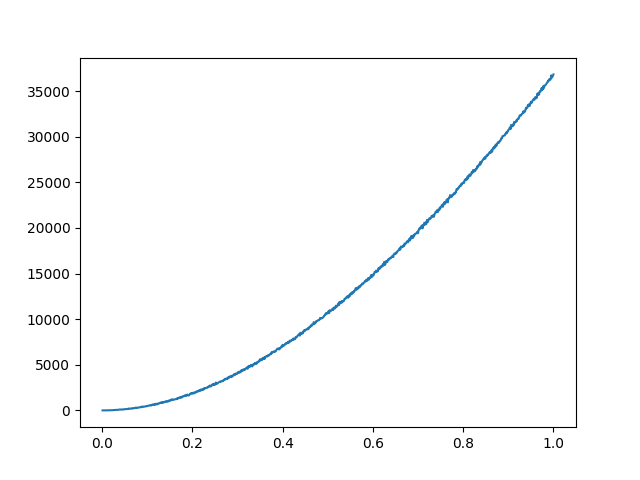
\includegraphics[scale=0.75]{collisioni_concatenamento.png}
\captionof{figure}{Collisioni con fattore di carico < 1 gestite con concatenamento}

\subsubsection{Indirizzamento aperto}
Di seguito viene riportata una parte della tabella dei dati usata per il grafo del conteggio delle collisioni con indirizzamento aperto

\begin{tabular}{ |p{3cm}||p{3.5cm}|  }
 \hline
 \multicolumn{2}{|c|}{Collisioni gestite con indirizzamento aperto} \\
\hline
 $\alpha $ = 0.2 & 2564\\\hline
 $\alpha $ = 0.4 & 13765    \\\hline
 $\alpha $ = 0.6 & 46254 \\\hline
 $\alpha $ = 0.8 & 160822\\\hline
 $\alpha $ = 1 & 25981120  \\
 \hline
\end{tabular}

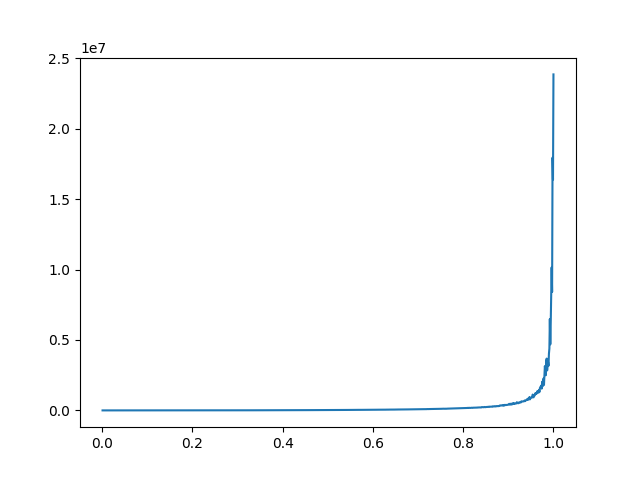
\includegraphics[scale=0.75]{collisioni_indirizzamento_aperto.png}
\captionof{figure}{Collisioni con fattore di carico < 1 gestite con indirizzamento aperto}

\subsection{Conclusioni}
Come previsto la differenza di collisioni nei due metodi di gestione delle tabelle risulta elevata. 

L'indirizzamento aperto, come evince dall'analisi teoria, risulta essere efficace con un fattore di carico intorno al 0,80, in quanto una volta che la tabella hash è arrivata a regime (è piena) e si vuole aggiungere un nuovo elemento quest'ultimo genererà al più m-1 collisioni (m dimensione della tabella) dato che si sta utilizzando una funzione hash lineare. Dal grafico si può anche notare un andamento praticamente esponenziale delle collisioni a partire dal valore 0,8.

Nella gestione delle collisioni con concatenamento possiamo notare un andamento di esse abbastanza lineare in quanto la dimensione della tabella risulta essere "infinita" e ad ogni inserimento possiamo avere al più una collisione.

\end{document}
